% -%-%-%-%-%-%-%-%-%-%-%-%-%-%-%-%-%-%-%-%-%-%-%-%-%
% MDI224 % 
% Data:12/12/2011                                 %
% Paris,France                                    % 
% Groupe:                                         %
% - Tiago Chedraoui Silva                   % 
% - Anthony CLERBOUT
% -%-%-%-%-%-%-%-%-%-%-%-%-%-%-%-%-%-%-%-%-%-%-%-%-%

\documentclass[a4paper,11pt]{article}

\usepackage[francais,listings,algo]{tcs}

% Cover %
\def \ttprofname{Roland BADEAU} % teachers name
\def \ttabrv{MDI224} % abbreviation of names class
\def \ttabrvxt{} % period
\def \mytitle{Interpolation par splines cubiques} % Big title
\def \mysubtitle{ Travaux Pratique 2 - Deuxième semestre de 2011} % subtitle
\def \ttauthi{Anthony CLERBOUT} % author's name
\def \ttxti{Casier: 234} % Extra text right side of name
\def \ttauthii{Tiago CHEDRAUOI SILVA} % author's name
\def \ttxtii{Casier: 214 } % Extra text right side of name
\def \ttdate{Décembre 15, 2011} % date

\begin{document}
\titleTMB 
\newpage
\tableofcontents
\listoffigures
\newpage

\section{Résolution du système linéaire}

\subsection{Méthode de relaxation}
Nous pouvons exprimer analytiquement la valeur de $x_i^{k+1}$

\begin{eqnarray*}
  J(x) 	&=& \frac{1}{2} x^TAx - x^Tb\\
        &=& \frac{1}{2} \sum_{i}\sum_{j} x_i^{k+1}x_j^{k+1}a_{ij} - \sum_{i} x_i^{k+1}b_i\\
\frac{\delta J}{\delta x_i^{k+1}} &=& \sum_{j\leq i} x_j^{k+1}a_{ij} + \sum_{j>i} x_j^{k} a_{ij} - b_i = 0\\
x_i^{k+1} &=& \frac{1}{a_{ij}} (b_i - \sum_{j<i} x_j^{k+1}a_{ij} - \sum_{j>i} x_j^{k} a_{ij})
\end{eqnarray*}

On  observe  qu'il  s'agit  de l'expression  de  $x_i^{k+1}$  dans
l'algorithme de  Gauss-Seidel et également  dans l'algorithme de
relaxation avec w=1.

\subsection{Méthode du gradient à pas constant}

\subsubsection{Complexité}
A chaque itération on fait:
$ g = A*x_n-b$ et $   xn = x(:,i+1)-beta*g$
Donc: Comme A est une matrice tridiagonal, $A*x_n$ fait 3N multiplications, et 
$beta*g$ fait N. Donc, on a 4N multiplication a chaque itération pour la méthode
du gradient à pas constant.


Pour  le méthode  de relaxation  on  fait:$x_i^{k+1} =  \frac{1}{a_{ij}} (b_i  -
\sum_{j<i}  x_j^{k+1}a_{ij} - \sum_{j>i}  x_j^{k} a_{ij})$,  et cela  nous donne
aussi 4N multiplications.


\subsubsection{Convergence de l'algorithme}
On pose $e^{n+1}=x^{n} - x^{*}$. On a donc:
\begin{eqnarray*}
  e^{n+1} &=& x^{n+1}-x^{*}\\ 
  &=& x^{n}-\beta(Ax^{n}-b) - x^{*}\\
  &=& (I_n-\beta A) e^{n}
\end{eqnarray*}


On sait qu'il  existe une base orthonormale de vecteurs propres  de A, notons là
$(p_i)_{1\leq i\leq N}$
Soit v appartenant à $R^{n}$, on pose $v = sum_{i=1}^N{v_i . p_i}$

On a alors : 

\begin{eqnarray*}
  (I_n - \beta A) v &=& \sum_{i=1}^N (I_n-\beta A) v_i p_i\\
  & =& \sum_{i=1}^N(1-\beta \lambda_i) v_i p_i
\end{eqnarray*}


Ainsi :

\begin{eqnarray*}
  ||I_n - \beta A ||^2_2 	&=& (\sum_{i=1}^N(1-\beta \lambda_i) v_i p_i,\sum_{j=1}^N(1-\beta \lambda_j) v_j p_j)\\
  &=& \sum_{i=1}^N(1-\beta \lambda_i^2) v_i^2\\
  &\leq& max (1-\beta \lambda_i) \sum_{j=1}^N v_j^2 = (max |1-\beta \lambda_i|^2 * ||v||_2^2)
\end{eqnarray*}

Pour tout v appartenant à $R^n$, on a donc:

\begin{eqnarray*}
  ||e^{n+1}||_2 \leq max |1-\beta \lambda_i| ||e^n||_2
\end{eqnarray*}

On note $\rho (b) = max |1-\beta \lambda_i|$
et par récurrence, on obtient:

\begin{eqnarray*}
  ||e^{n}||_2 \leq \rho(B) ||e^0||_2
\end{eqnarray*}


On doit donc vérifier que $\rho (B) < 1$!

Pour tout $i \in [1,N]:$ :
\begin{eqnarray*}
  \lambda_N\leq\lambda_i\leq\lambda_1.
\end{eqnarray*}


Donc:
\begin{eqnarray*}
  1-\beta \lambda_1\leq1- \beta \lambda_i\leq 1 - \beta \lambda_N
\end{eqnarray*}

Donc:

\begin{eqnarray*}
  \rho (B) = max |1-\beta \lambda_i| = max (|1-\beta \lambda_1|, max |1-\beta \lambda_N|)
\end{eqnarray*}

L'algorithme converge seulement si $\rho(B)<1$.

Donc $|1-\beta \lambda_1|<1$ est équivalent à : 

\begin{eqnarray*}
  1-\beta \lambda_1<1\; \text{et} \; \beta \lambda_1-1<1& \\
  \text{Soit } 0<\beta<\frac{2}{\lambda_1}.&
\end{eqnarray*}


\begin{figure}[h!]
  \begin{centering}
    \includegraphics[scale=0.5]{../conv_beta}
    \label{rspro2}
    \par\end{centering}
  \caption{Taux de convergence de la méthode gradient en fonction de beta: théorique}
  \label{fig:jacobi-conv}
\end{figure}

On     a    trouvé     $\lambda_N=1.4384$     et    $\lambda_1=5.5616$,     donc
$\beta_{optimal}=\frac{2}{7}$.  Cette  valeur est plus  petite que la valeur du
taux de convergence de la méthode de relaxation : $w_{optimal}=1.1$.  


\subsubsection{Taux de convergence optimal}

Premièrement,$\rho(B)=\text{taux de  convergence}$ et la  vitesse de convergence
du gradient à pas fixe est $-ln(\rho(B))$.

Comme $\rho(B) = max(1-\beta \lambda_n,\beta\lambda_1-1)$ .
Donc $\rho(B)$ est minimale lorsque $1-\beta\lambda_n=\beta\lambda_1-1$

Soit: $\beta=\beta_0=\frac{2}{\lambda_1+\lambda_n}$

\begin{eqnarray*}
  \rho(B)&=&\frac{\lambda_1-\lambda_n}{\lambda_1+\lambda_n}
\end{eqnarray*}



D'où quand N est grand, la vitesse de convergence est :
\begin{eqnarray*}
  -ln(1-\frac{2\lambda_n}{\lambda_1+\lambda_n})=-ln(1-\frac{2}{1-k}) &\text{Avec } k=\frac{\lambda_1}{\lambda_n}&.
\end{eqnarray*}

\subsubsection{Implémentation}

Pour voir la méthode du gradient à pas constant, on a fait le code suivant:

\begin{multicols}{2}
  \lstinputlisting[title=\textbf{Méthode du gradient à pas constant}]{../mygradient.m}
\end{multicols}

Losqu'on l'utilise, on trouve comme solution:

\begin{center}
  $x = [ 0.99996 \; 1.00002 \; 0.99998 \; 1.00002 \; 0.99996]^T$
\end{center}

Cette solution n'est pas optimale, mais est beaucoup proché de la solution opimale
($x^* = [ 1.0 \; 1.0 \; 1.0 \; 1.0 \; 1.0]^T$
);

\subsubsection{Variation du taux de convergence}

\begin{figure}[h!]
  \begin{centering}
    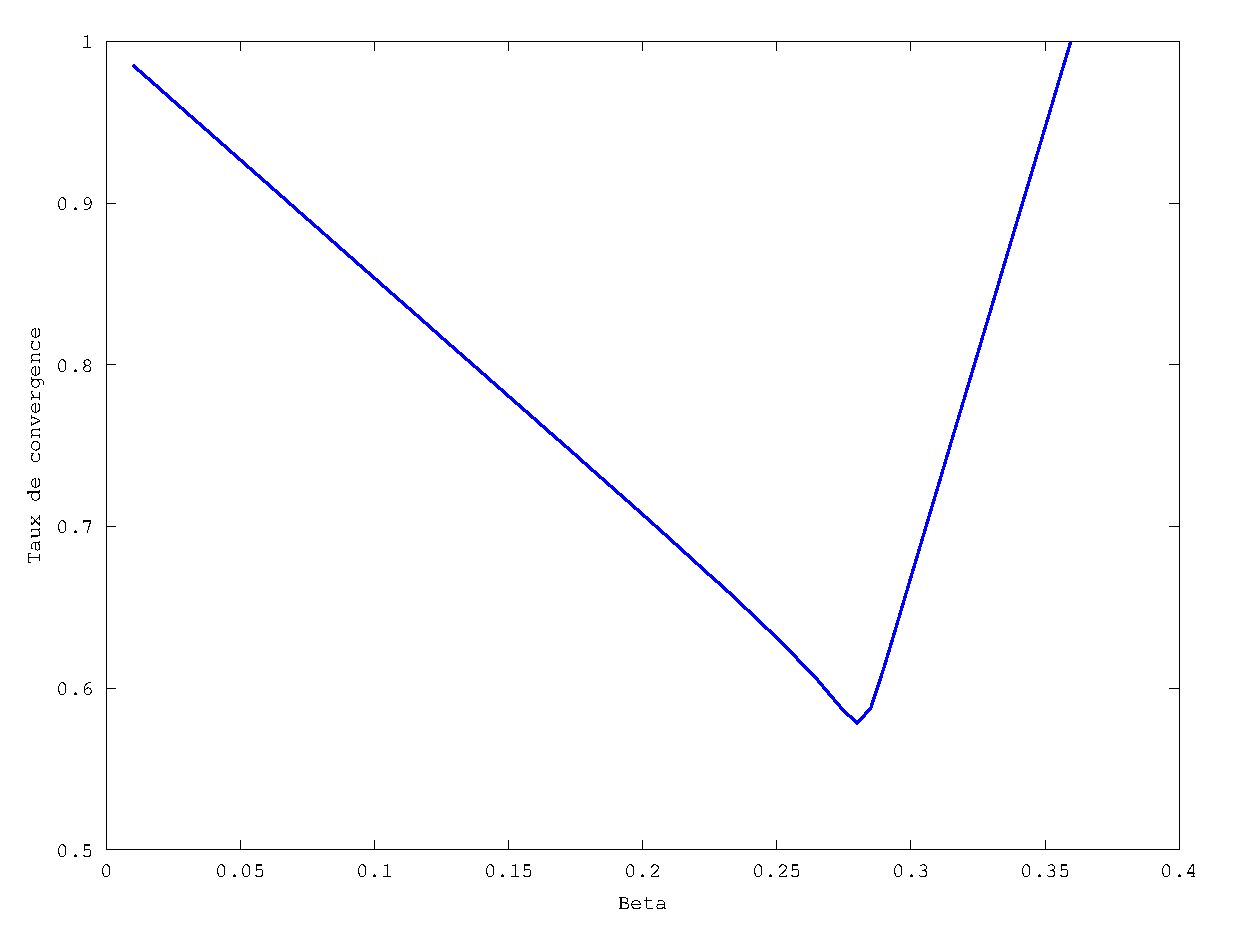
\includegraphics[scale=0.5]{../grad_beta}
    \label{rspro2}
    \par\end{centering}
  \caption{Taux de convergence de la méthode gradient en fonction de beta: réel}
  \label{fig:jacobi-conv}
\end{figure}

\newpage
\subsection{Méthode du gradient à pas optimal}

\subsubsection{$\beta$ qui minimise $J(x_k)-\beta g_k$}

Pour trouver $\beta$ qui minimise $J(x_k)-\beta g_k$,
avec $g_{k+1}=-\nabla J(x_k+\beta_kg_k)$.

Soit:
\begin{eqnarray*}
  f'(\beta_k)= 0 &=& (\nabla J(x^k+\beta_kg_k),g_k)\\
  &=&-(g_{k+1},g_k)=-g_{k+1}^Tg_k
\end{eqnarray*}

On a $g_{k+1}= b -Ax_k-\beta_kAg_k=g_k-\beta_kAg_k$

Donc :
\begin{eqnarray*}
  (g_{k+1},g_k) = 0  &\Rightarrow&  (g_k-\beta_kAg_k,g_k)  = 0\\
  & \Leftrightarrow& (g_{k},g_k)-\beta_k(Ag_k,g_k) = 0\\
  & \Leftrightarrow&  \beta_k=\frac{(g_{k},g_k)}{(Ag_k,g_k)}= \frac{(g_{k}^T,g_k)}{g_k^TA^Tg_k}
\end{eqnarray*}

\subsubsection{Complexité}

Pour cette méthode on fait: 
  $g = A*xn-b$, 3N multiplications, et après 
 $ beta = g'*g/(g'*A*g)$, 6N multiplications, et enfin $ xn = x(:,i+1)-beta*g$, N multiplications. Donc, on a 10N.

Ce coût est plus grand que le coût des valeurs antérieures.

\subsubsection{Implémentation}
Pour voir la méthode du gradient à pas optimal, on a fait le code suivant:

\begin{multicols}{2}
  \lstinputlisting[title=\textbf{Méthode du gradient à pas optimal}]{../gradient_optimal.m}
\end{multicols}


\subsubsection{Taux de convergence}
\begin{figure}[h!]
  \begin{centering}
    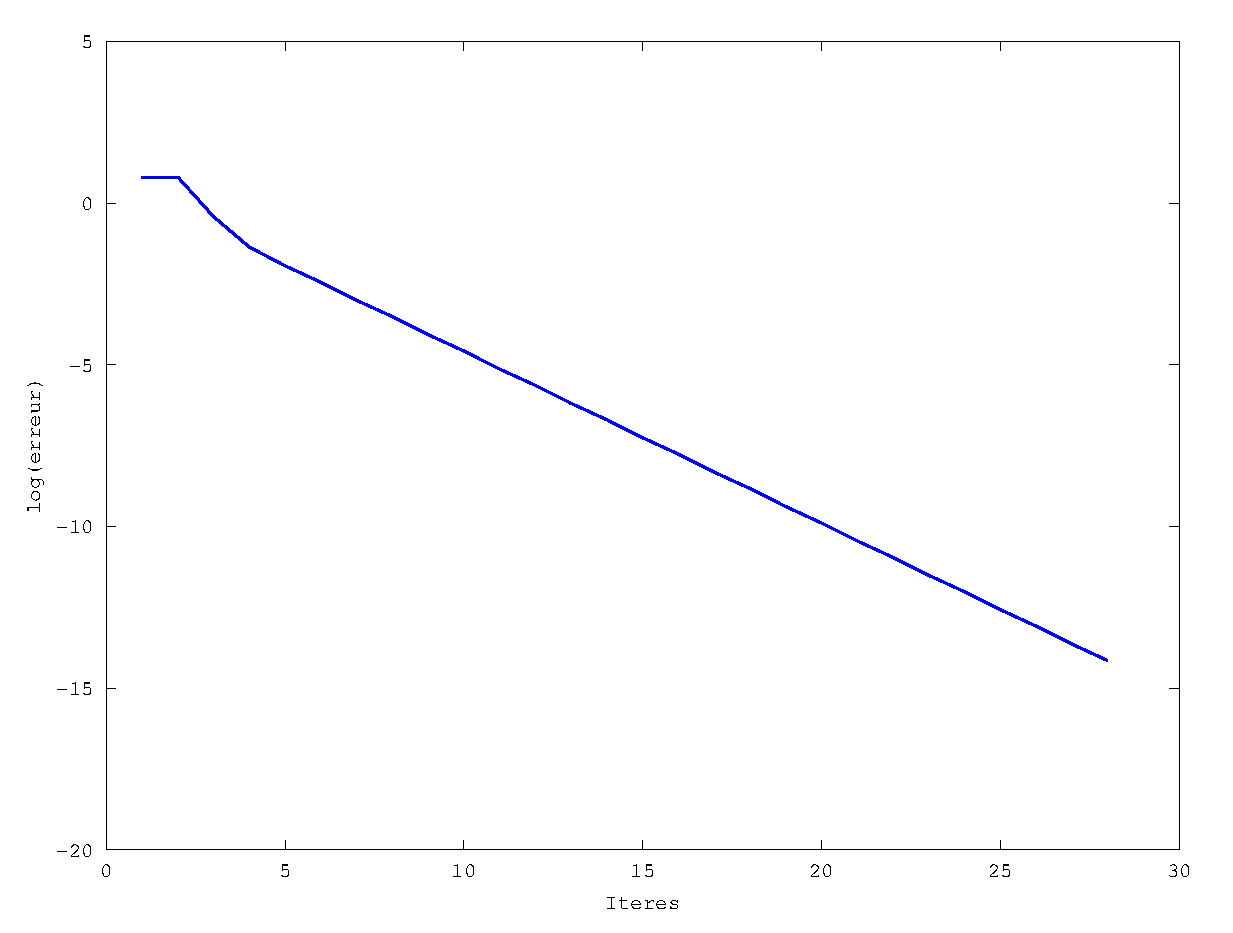
\includegraphics[scale=0.5]{../grad_optimal}
    \label{rspro2}
    \par\end{centering}
  \caption{Convergence de la méthode gradient optimal}
  \label{fig:jacobi-conv}
\end{figure}

En utilisant la fonction polyfit de Matlab, on a trouvé $\text{p(x)= -0.547007 x
  + 1.029611 }$. Donc, le taux de convergence de
l’algorithme trouvée est: -0.54.

L'intéret d'avoir le $\beta$ optimal est que l'algorithme converge plus rapidement.

\subsection{Méthode du gradient conjugué}

\subsubsection{Complexité}
Le nombre d´itérations de cet algorithme est proportionnel à la taille n de la matrice du système. Cela veut dire que le gradient conjugué converge au plus n itérations.
Pour une matrice pleine, la méthode demande $2n^3$ opérations mais comme la matrice
est creuse, la méthode fera moins que $2n^3$  opérations.

Pour la complexité on fait:
$ beta = g'*w/(w'*A*w);$ 6N multiplications,
$ xn = x(:,i+1)-beta*w;$ N multiplications,
$ g = A*xn-b;$ 3N multiplications,
$ a = -g'*A*w/(w'*A*w);$ 7N multiplications,
$ w=g+a*w;$ N multiplications,

Donc: 15  multiplications. Cela est la  plus grand des complexités  de touts les
autres algorithmes, on perd en
complexité, mais on gagne grâce au nombre d'itérations qui est le plus petit.

\subsubsection{Implémentation}

Pour voir la méthode du gradient conjugé, on a fait le code suivant:

\begin{multicols}{2}
  \lstinputlisting[title=\textbf{Méthode du gradient conjugué}]{../gradient_conjugue.m}
\end{multicols}


\subsubsection{Temps d'exécution}

\begin{table}[h!]
  \begin{center}
    \begin{tabular}{|c|c|}
      \hline 
      Méthode & Temps \\
      \hline 
      \hline 
      Gradient conjugué & 0.0017250 s\\
      Relaxation & 0.0044890\\
      Gradient optimal & 0.0044729 s\\
      \hline 
    \end{tabular}
  \end{center}
  \caption{Comparatif des temps d´éxécution de différentes méthodes de
    résolution linéaire}
\end{table}


\subsection{Application }

\begin{multicols}{2}
  \lstinputlisting[title=\textbf{Calcul de spline cubique naturelle}]{../tstinvtridiag0.m}
\end{multicols}



\begin{figure}[h!]
  \begin{centering}
    \subfigure[Example 1]{
      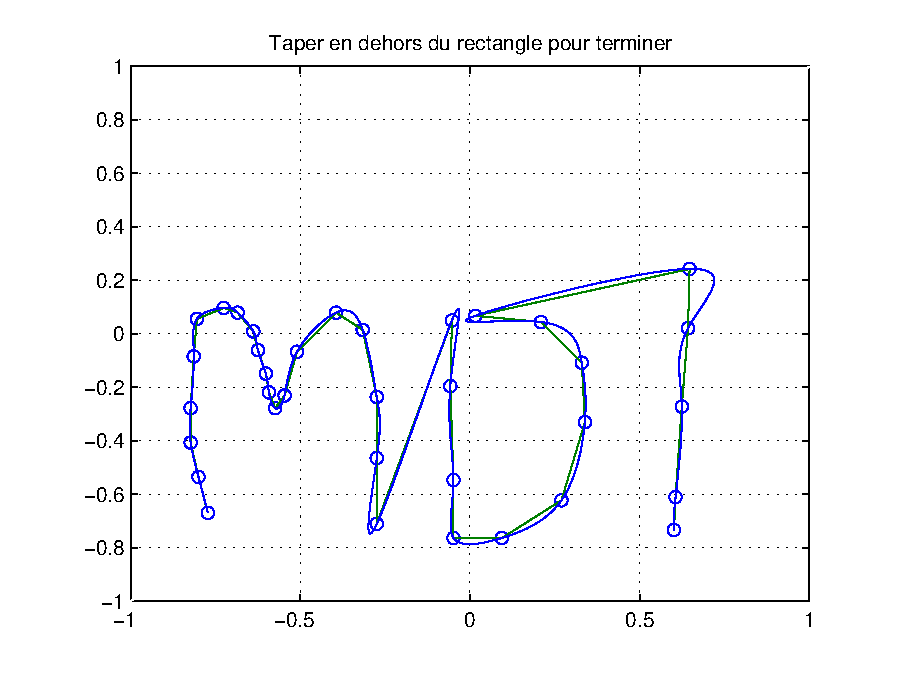
\includegraphics[scale=0.35]{../figue_spline3}}  
    \subfigure[Example 2]{
      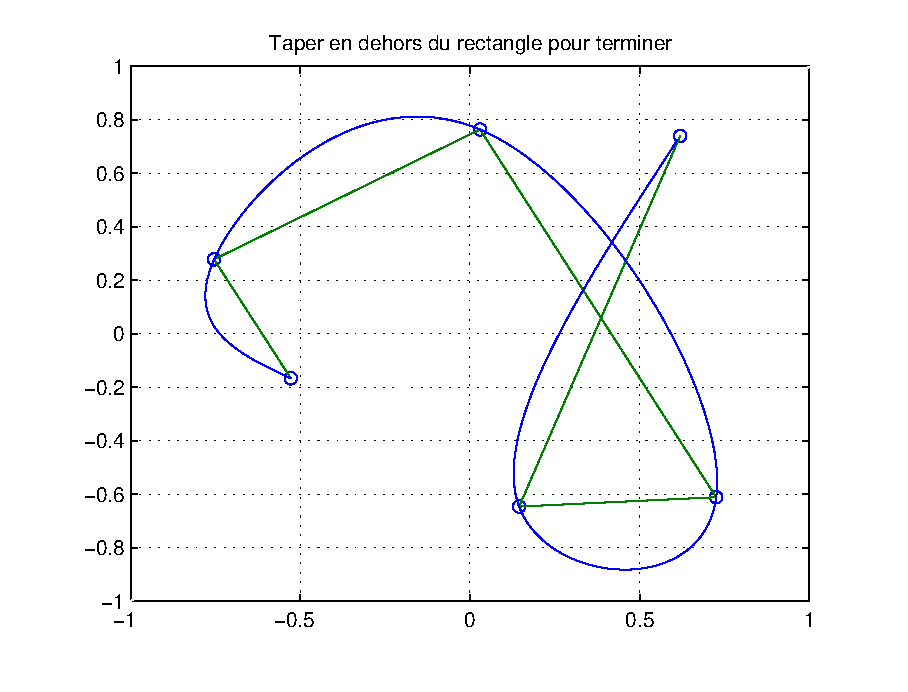
\includegraphics[scale=0.35]{../exemple_spline_naturelle}
    }
    \par\end{centering}
  \caption{Calcul de spline cubique naturelle}
  \label{rspro}
\end{figure}

\end{document}

